\documentclass[11pt,oneside,openany,report]{jsbook}

\usepackage[a4paper,truedimen,margin=25truemm]{geometry}
\usepackage{cscover}
\usepackage[dvipdfmx]{graphicx}
\usepackage[nobreak]{cite}
\usepackage[a4paper,dvipdfmx,pdfdisplaydoctitle=true,%
    bookmarks=true,bookmarksnumbered=true,bookmarkstype=toc,bookmarksopen=true,%
    pdftitle={学位論文の体裁に関する研究},%
    pdfauthor={東工大太郎}%
    ]{hyperref}
\usepackage{pxjahyper}

\renewcommand{\bibname}{参考文献}
\setcounter{tocdepth}{2}
\pagestyle{plain}

\newcommand{\TODO}[1]{\textbf{[TODO: #1]}}
%\renewcommand{\TODO}[1]{}

\thesistype{学士特定課題研究論文}
\title{学位論文の\\体裁に関する研究}
\author{東工大 太郎}
\studentid{17B00000}
\affiliation{東京工業大学\\情報理工学院\\情報工学系} 
\date{2021年1月}

\supervisorname{指導教員}
\supervisor{情報 一郎}
%\dsupervisorname{副指導教員}
%\dsupervisor{工学 次郎}

\begin{document}

\frontmatter
\maketitle

\chapter{概要}
学士特定課題研究論文は、シングルカラムでページ数に制限はない。

\tableofcontents
\listoffigures
\listoftables

%%%%%%%%%%%%%%%%%%%%%%%%%%%%%%%%%%%%%%%%%%%%%%%%%%

\mainmatter
\chapter{序論}
本論文は、学士特定課題研究論文の書き方\cite{tokodai-xyz2015}の一例を示す。

\section{本研究の位置づけ}
ここでは、色々なサンプルを示す。
次の式(\ref{eq:hs})の通り$n$次元の超球を仮定する。
$n=3$の場合は図\ref{fig:hs}のようになる。
\begin{equation}
  r^2 = \sum_{k=1}^{n} x_k^2 \label{eq:hs}
\end{equation}
\begin{figure}[tb]
  \centering
  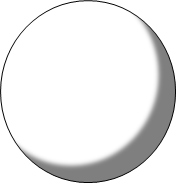
\includegraphics[scale=1.0]{fig/sample.png}
  \caption{3次元の球}\label{fig:hs}
\end{figure}

一方で、表\ref{tab:sample}によれば、a、b、c、dの4つの要素がある。
\begin{table}[tb]
  \centering
  \caption{要素群}\label{tab:sample}
  \begin{tabular}{|c|r|}
    \hline
    a & b \\ \hline
    c & d \\ \hline
  \end{tabular}
\end{table}

%%%%%%%%%%%%%%%%%%%%%%%%%%%%%%%%%%%%%%%%%%%%%%%%%%

\chapter{結論}
結論は、網羅的にかつ簡潔に。

%%%%%%%%%%%%%%%%%%%%%%%%%%%%%%%%%%%%%%%%%%%%%%%%%%

\appendix
\chapter{定理1の証明}
必要に応じて、付録を載せる。

%%%%%%%%%%%%%%%%%%%%%%%%%%%%%%%%%%%%%%%%%%%%%%%%%%

\backmatter
\chapter{謝辞}
本論文の執筆にあたり、議論して頂いた関係者に感謝する。

%%%%%%%%%%%%%%%%%%%%%%%%%%%%%%%%%%%%%%%%%%%%%%%%%%

\bibliographystyle{jplain}
\bibliography{references}
%\begin{thebibliography}{99}
%  \bibitem{tokodai-xyz2015} 東工大太郎. 良い論文の書き方. \textit{Journal of XYZ}, Vol.~3, No.~4, pp. 15--34, 2015.
%\end{thebibliography}

\end{document}
